\chapter*{Appendix}
\addcontentsline{toc}{chapter}{Appendix}
\section*{Fresnel Propagation Model}
In this section, we will briefly discuss the Fresnel propagation model used for obtaining the effects of diffraction. The model is based on \cite{FourierOptics} and the MATLAB model developed at Optica Group was used.  The fresnel number for the system is given by the equation
\begin{equation}
N_F = w^2/(\lambda z)
\label{eq:fresnel-4}
\end{equation}

where $w$ is the half-width of the square aperture, $\lambda$ is the wavelength, and $z$ is the distance between the source plane and the object plane. In the simulations, $\lambda$ was taken to be 550 nm, since the average wavelength of the visible light spectrum is 550 nm. The distance $z$ is taken to be 5 mm. $w$ is basically the pixel size(assumed to be $2.2 \mu m \times 2.2 \mu m$) of the mask plane multiplied by the total number of openings in the aperture. The simulation assumes that the sensor reacts to only one specific wavelength and that signals from other wavelength sources are ignored. The fresnel number depends on the source plane(i.e the mask). For a single pinhole system, the fresnel number is 0.044 and for a doubly-toeplitz mask of size $1024 \times 1024$, it would be 20.34. It can be safely be assumed that the system lies in the fresnel region for this specific condition for this specific fresnel number range\cite{FourierOptics} as the system still does not reach far-field region. When modeling the diffraction effect, we have a source plane and an observation plane. In our case, the source plane is the mask and the observation plane would be the sensor. This is shown in Figure \ref{fig:fresnel_1}. 
\begin{figure}[!htbp]
\centering
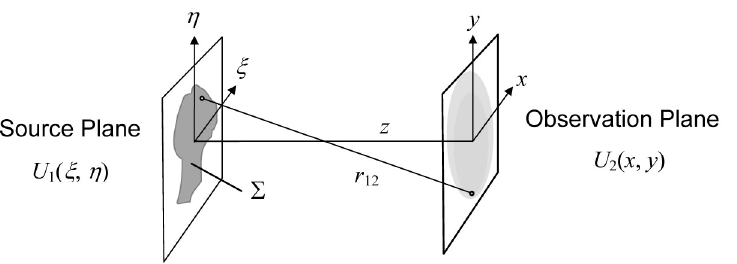
\includegraphics[width = \linewidth]{pics/fresnel-1}
\caption{Source Plane and Observation Plane}
\label{fig:fresnel_1}
\end{figure}
In this case, the diffraction effects can be given by the equation \ref{eq:fresnel-1}.

\begin{equation}
\label{eq:fresnel-1}
U_2(x,y) = \frac{e^{jkz}}{j\lambda z}\int \int U_1(\xi, \eta )exp(\frac{jk}{2z}[(x - \xi)^2 + (y - \eta)^2])d\xi d\eta
\end{equation}
This expression can also be written in the form of equation \ref{eq:fresnel-2}.
\begin{equation}
\label{eq:fresnel-2}
U_2(x,y) = F^{-1}(F(U_1(x,y)F(h(x,y)))
\end{equation}
where
\begin{equation}
\label{eq:fresnel-3}
h(x,y) = \frac{e^{jkz}}{j\lambda z}exp(\frac{jk}{2z}(x^2 + y^2))
\end{equation}

The mask transfer function for the binary mask is calculated using equation \ref{eq:fresnel-2}. This obtained pattern on the observation plane is then used in the place of the binary mask to simulate the effect of a diffracted mask. 
\section*{Camera Dimensions}
This section shows the dimension of the camera module as provided by the camera vendor. The measurements for the front side of the camera module is shown in Figure \ref{fig:arducam_mech}. The OV2640 and OV5642 cameras upon the lenses removed have a thickness of 4.29 mm and 2.70 mm respectively. The difference in thickness is due to the presence of AL422B FIFO Buffer chip which increases the thickness of the camera. The thickness is the sum of the length of the circuit board plus the memory buffer element(which protrudes the most out of the circuit board). The camera modules are shown in Figure \ref{fig:camera_modules}.

\begin{figure}[!htbp]
\centering
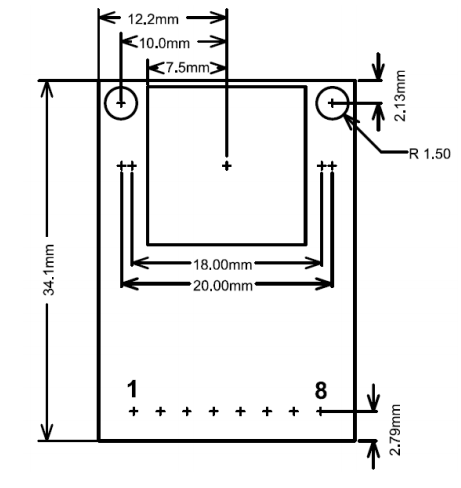
\includegraphics[width = 0.50 \linewidth]{pics/arducam_mech}
\caption{Dimensions of both OV5642 and OV2640 camera modules}
\label{fig:arducam_mech}
\end{figure}

\begin{figure}[ht]
\centering
    \begin{subfigure}{0.75\textwidth}
    \centering
        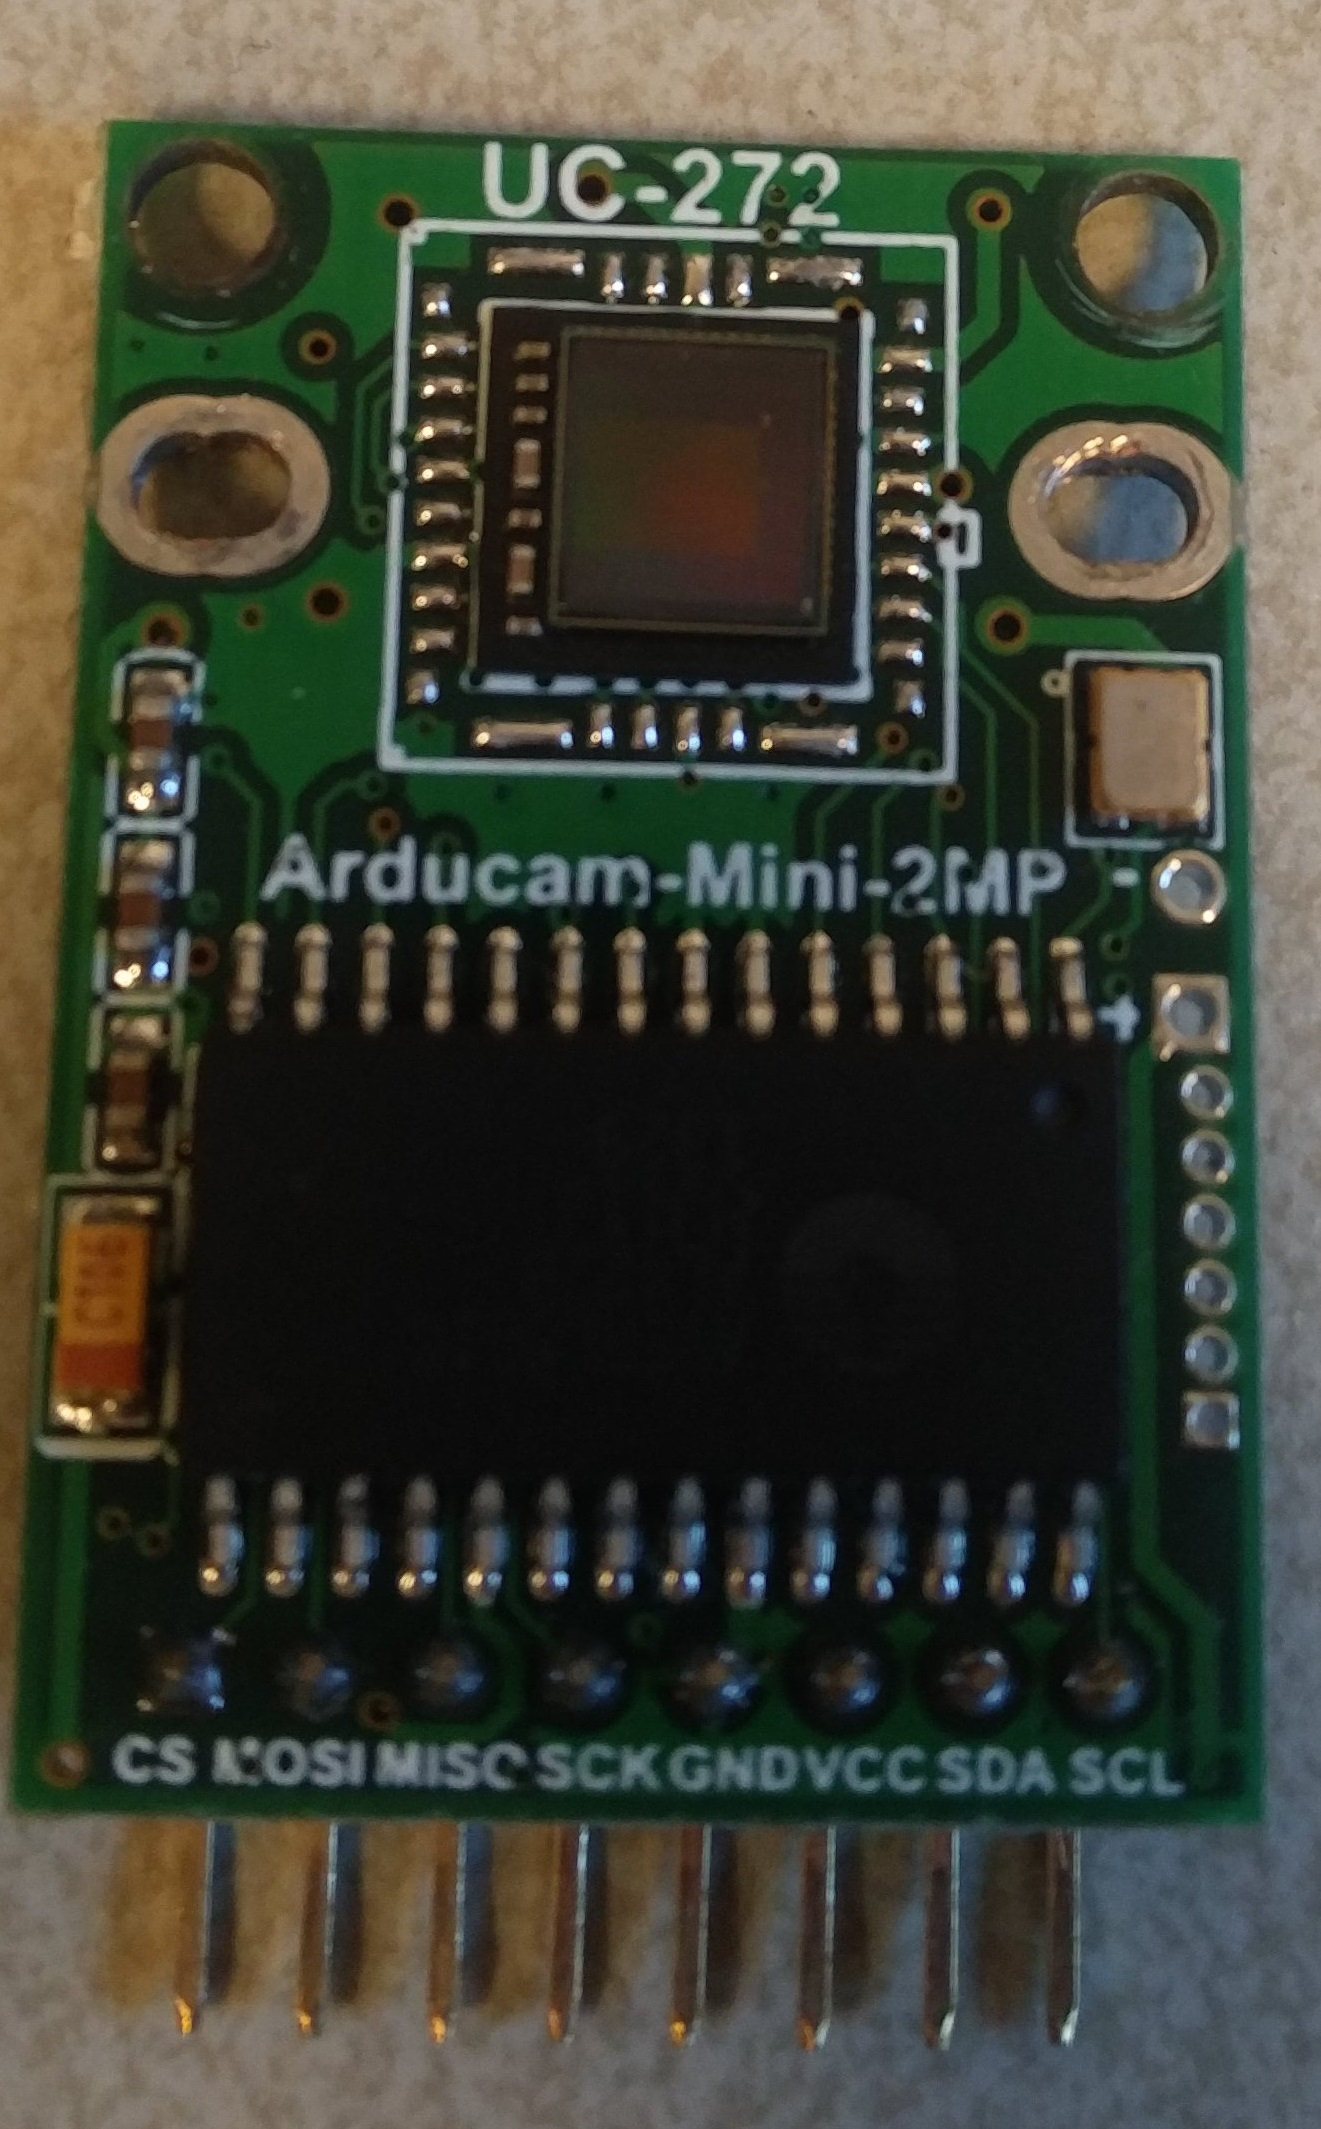
\includegraphics[width=0.25\linewidth]{pics/OV2640}
        \caption{OV2640 Camera Module}
    \end{subfigure}%
   
    \begin{subfigure}{\textwidth}
    \centering
        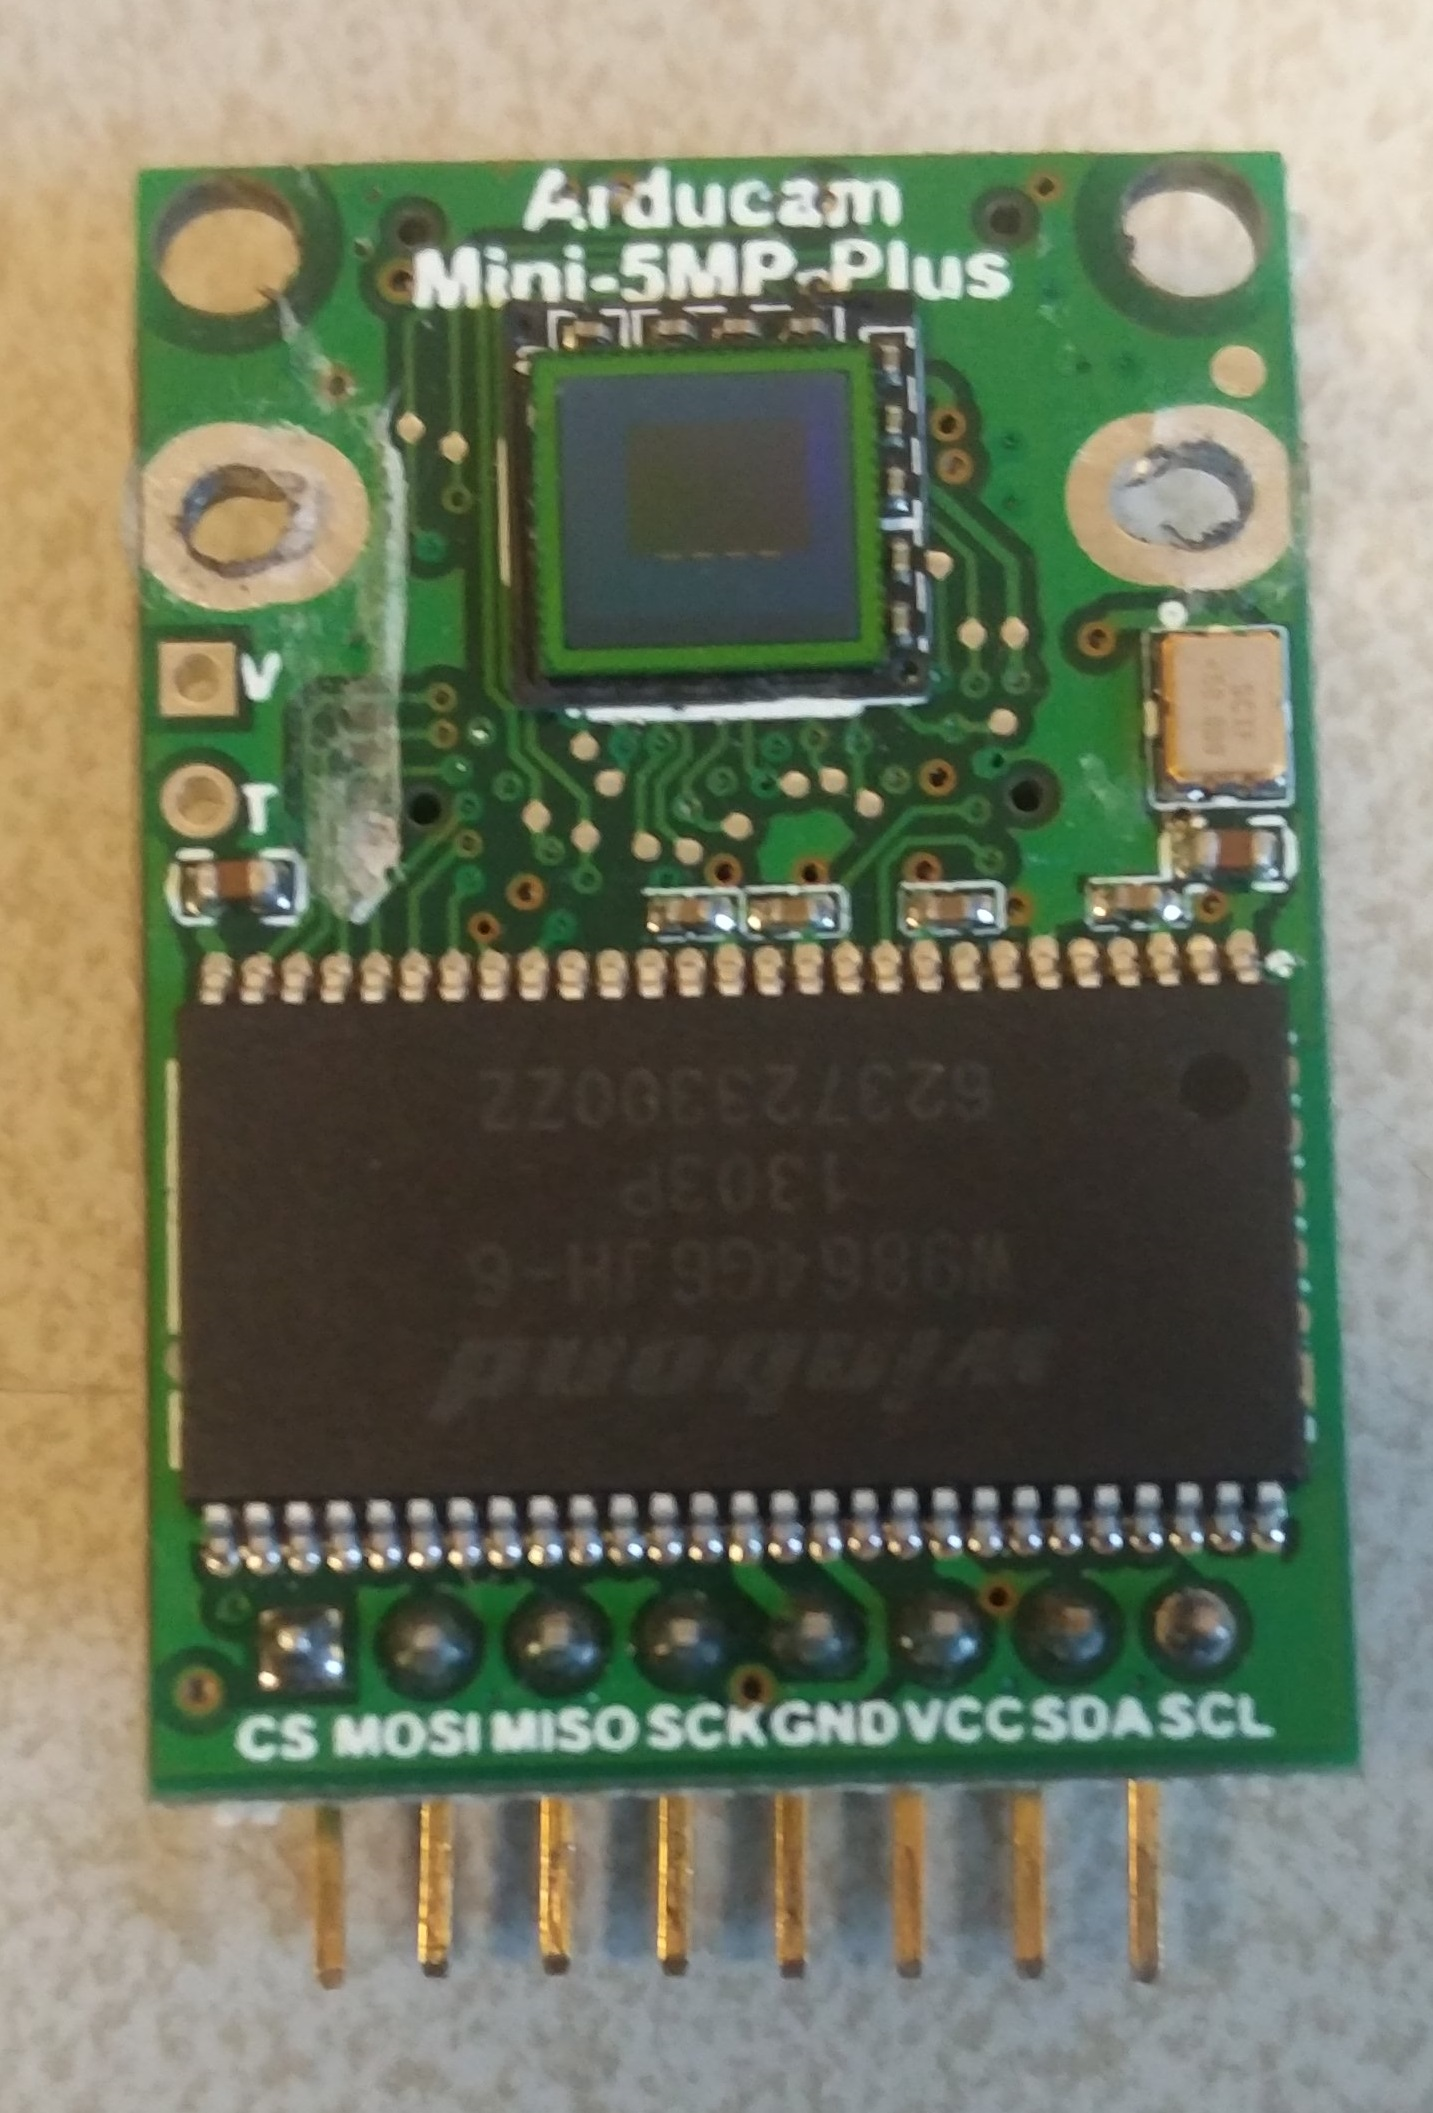
\includegraphics[width=0.25\linewidth]{pics/OV5642}
        \caption{OV5642 Camera Module}
    \end{subfigure}
       \caption{Camera Modules with lens removed}
        \label{fig:camera_modules}
   \end{figure}
   
   